\documentclass[14pt]{extarticle}
\usepackage{extsizes}
\usepackage[top=0.75in, bottom=0.5in, left=0.5in, right=0.5in]{geometry}
\usepackage{amsmath,amsfonts, color, booktabs, centernot, textcomp,amssymb,graphicx,verbatim,enumerate, bbm}
%\usepackage [autostyle, english = american]{csquotes}
%\usepackage [style = american]{csquotes}
%\MakeOuterQuote{"}
\usepackage{algorithm} % Boxes/formatting around algorithms
\usepackage[noend]{algpseudocode} % Algorithms
\usepackage{wrapfig}
\usepackage{fancyhdr}
\pagestyle{fancy}
\setlength\parindent{0pt}
\newcounter{problemnumber}
\def\Name{Leah Dickstein}  % Your name

\title{New Cost Function: Penalizing Large Control Power}
\author{\Name \vspace{-2ex}}
\date{\today}
\lhead{\Name}


\begin{document}
\maketitle

System: \\
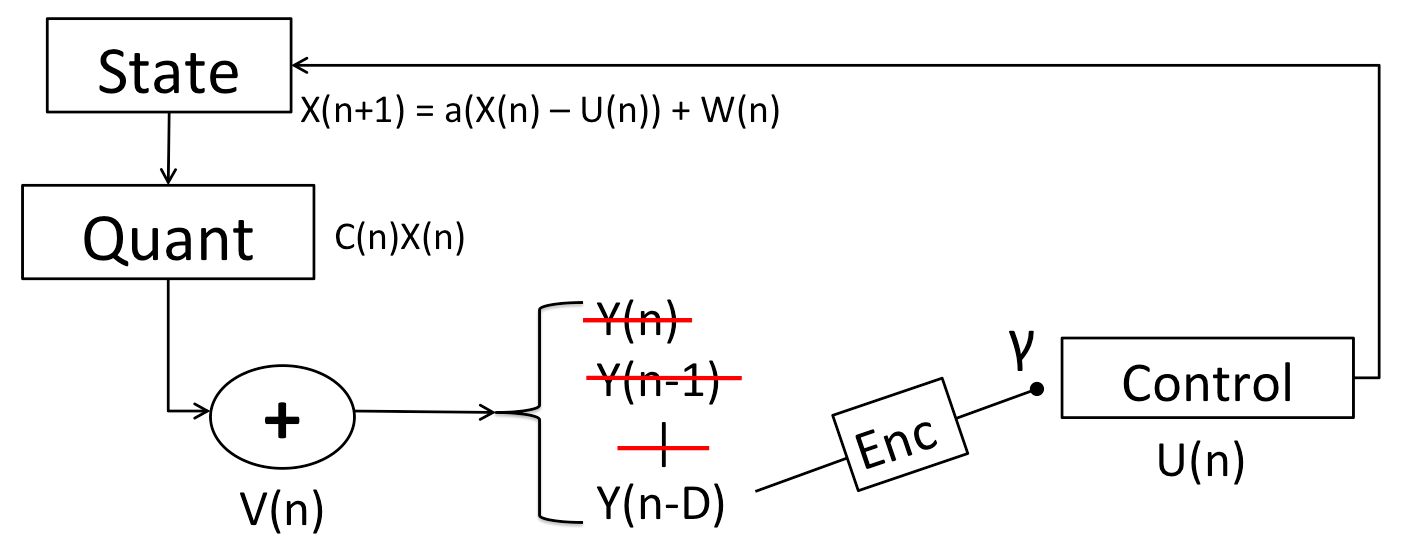
\includegraphics[width=0.5\textwidth]{sys_dynamics}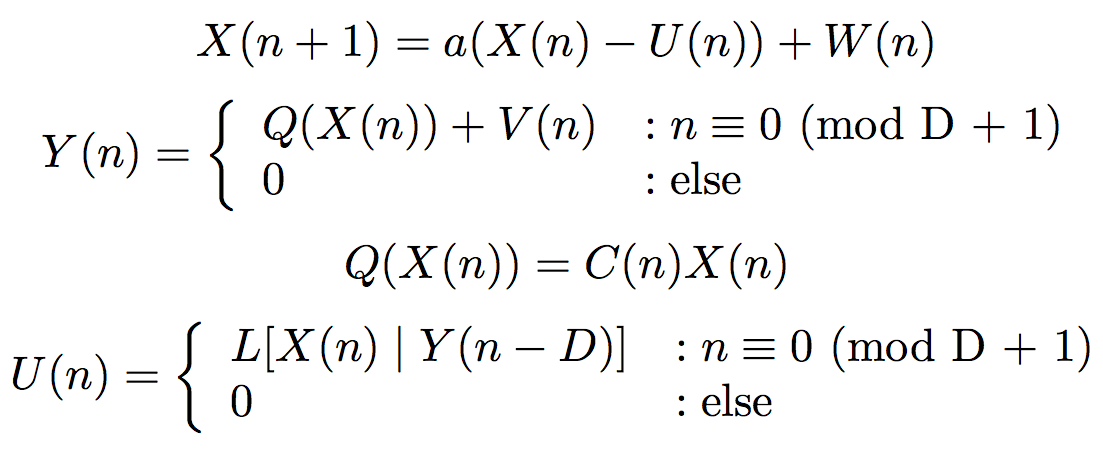
\includegraphics[width=0.5\textwidth]{sys_equations}
% 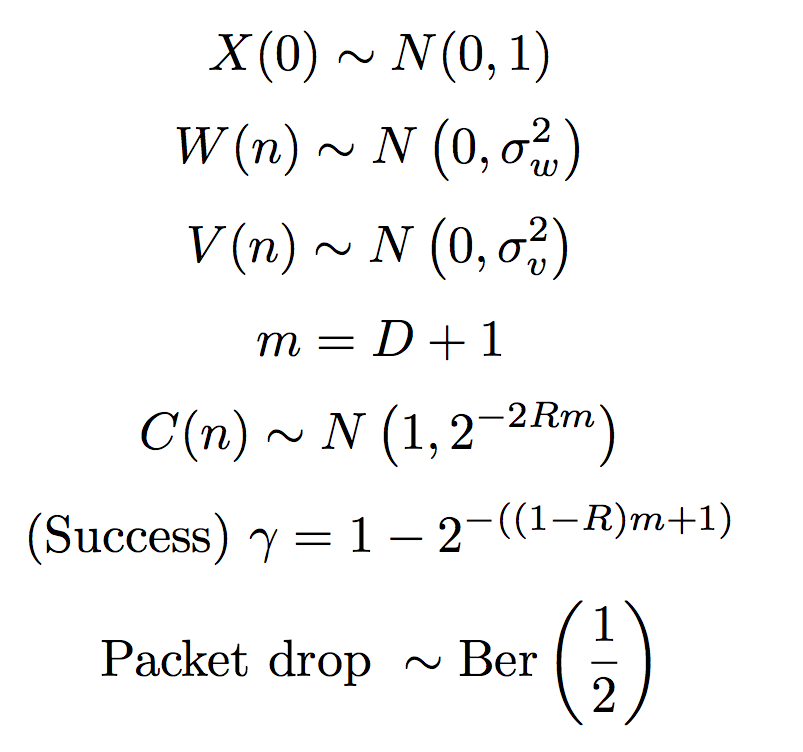
\includegraphics[width=0.35\textwidth]{sys_params}

\subsection*{New Cost Function -- No V(n)}

\[ \text{min } \mathbb{E} [ x^2(n+1) ] + \sum_{k=1}^n u^2(k) \]

\begin{math}
\text{min } \mathbb{E} [  a( x(n) - u(n) ) + w(n) )^2 ] + \sum_{k=1}^n u^2(k) \\
= \text{min } \mathbb{E} [( a( x(n) - \alpha y(n) ) + w(n) )^2 ] + \sum_{k=1}^n \alpha^2 y^2(k) \\
= \text{min } \mathbb{E} [( a( x(n) - \alpha c(n)x(n) ) + w(n) )^2 ] + \sum_{k=1}^n \alpha^2 c^2(k) x^2(k) \\
= \text{min } \mathbb{E} [ a^2 (1 - \alpha c(n) )^2 x^2(n) ] + \sigma_w^2 + \sum_{k=1}^n \alpha^2 u^2(k) \\
\frac{d}{d \alpha} \mathbb{E} [ a^2 (1 - \alpha c(n) )^2 x^2(n) ] + \sigma_w^2 + \sum_{k=1}^n \alpha^2 u^2(k) = \mathbb{E} [2a^2 (1 - \alpha c(n) ) (-c(n)) x^2(n) ] + \sum_{k=1}^n 2 \alpha u^2(k) = 0 \\
-a^2 ( \mu_c \sigma_{x(n)}^2 - \alpha (\mu_c^2 + \sigma_c^2 ) \sigma_{x(n)}^2 ) + \sum_{k=1}^n \alpha u^2(k) = 0 \\
\alpha (a^2 (\mu_c^2 + \sigma_c^2 ) \sigma_{x(n)}^2 + \sum_{k=1}^n u^2(k) ) = a^2 \mu_c \sigma_{x(n)}^2
\end{math}

\[ \alpha(n) = \frac{a^2 \mu_c \sigma_{x(n)}^2}{a^2 (\mu_c^2 + \sigma_c^2) \sigma_{x(n)}^2 + \sum_{k=1}^n u^2(k)} \]

This is easy to implement, and my next step is to implement this. My worry is that this isn't a closed solution like the previous $\alpha$ calculations. As time passes, $\alpha$ will change every time a new control is implemented--which is fine, but we should note the new complication. Does this answer make sense? Should I go ahead and implement this?

\subsection*{Original Cost Function -- No V(n)}

\[ \text{min } \mathbb{E} [x^2(n+1) ] \]
\[ u(n) = \alpha y(n) = \alpha c(n) x(n) \]

\begin{math}
\text{min } \mathbb{E} [( a( x(n) - u(n) ) + w(n) )^2 ] \\
= \text{min } \mathbb{E} [( a( x(n) - \alpha y(n) ) + w(n) )^2 ] \\
= \text{min } \mathbb{E} [( a( x(n) - \alpha c(n)x(n) ) + w(n) )^2 ] \\
= \text{min } \mathbb{E} [ a^2 (1 - \alpha c(n) )^2 x^2(n) ] + \sigma_w^2 \\
\frac{d}{d \alpha} \mathbb{E} [ a^2 (1 - \alpha c(n) )^2 x^2(n) ] + \sigma_w^2 = \mathbb{E} [2a^2 (1 - \alpha c(n) ) (-c(n)) x^2(n) ] = 0 \\
\mathbb{E} [c(n) x^2(n) - \alpha c^2(n) x^2(n) ] = 0 \\
\mu_c \sigma_{x(n)}^2 = \alpha (\mu_c^2 + \sigma_c^2 ) \sigma_{x(n)}^2
\end{math}

\[ \alpha = \frac{\mu_c}{\mu_c^2 + \sigma_c^2} \]

These are the results we expect, from Gireeja's Noncoherence Paper.

\subsection*{Original Cost Function}

\[ \text{min } \mathbb{E} [x^2(n+1) ] \]

\begin{math}
\text{min } \mathbb{E} [ ( a(1-\alpha c(n) ) x(n) - a\alpha v(n) + w(n) )^2 ] \\
= \text{min } \mathbb{E}[ a^2 (1-\alpha c(n) )^2 x^2(n) + \mathbb{E} [a^2 \alpha^2 v^2(n) ] + \sigma_w^2 \\
\frac{d}{d \alpha}  \mathbb{E}[ a^2 (1-\alpha c(n) )^2 x^2(n) + \mathbb{E} [a^2 \alpha^2 v^2(n) ] + \sigma_w^2 = \mathbb{E}[ -2a^2 (1-\alpha c(n)) c(n) x^2(n) ] + 2 a^2 \alpha \sigma_v^2 = 0\\
= -\mu_c \sigma_{x(n)}^2 + \alpha (\mu_c^2 + \sigma_c^2 ) \sigma_{x(n)}^2 + \alpha \sigma_v^2 = 0
\end{math}

\[ \alpha(n) = \frac{\mu_c \sigma_{x(n)}^2}{(\mu_c^2 + \sigma_c^2) \sigma_{x(n)}^2 + \sigma_v^2} \]

These are the results we expect from the LLSE theorem: $\alpha = \frac{cov(X, Y)}{var(Y)} = \frac{\mathbb{E}[XY]}{\mathbb{E}[Y^2]} \leftarrow \text{assuming } \mathbb{E}[X] = \mathbb{E}[Y] = 0 $

\end{document}